\documentclass[a4paper,10pt]{article}


\usepackage{epsfig}
\usepackage{subfigure}
\usepackage{calc}
\usepackage{amssymb}
\usepackage{amstext}
\usepackage{amsmath}
\usepackage{amsthm}
\usepackage{multicol}
\usepackage{pslatex}
\usepackage{apalike}
% Please add other packages that you may need BEFORE the SCITEPRESS.sty package.
\usepackage{xcolor}
%%%%%%%%%%%%%%%%%%%%%%%%%%%%%%%%%%%%%%%%%%%%%%%%%%%%%%%%%%%%%%%%%%
\usepackage{SCITEPRESS}

\subfigtopskip=0pt
\subfigcapskip=0pt
\subfigbottomskip=0pt

%%%%%%%%%%%%%%%%%%%%%%%%%%%%%%%%%%%%%%%%%%%%%%%%%%%%%%%%%%%%%%%%%%
\newcommand{\TODO}[1]{\begingroup\color{red}#1\endgroup}
\newcommand{\PFS}[1]{\begingroup\maybecolor{green}#1\endgroup}
\newcommand{\NR}[1]{\begingroup\maybecolor{Orange}#1\endgroup}
\newcommand{\FK}[1]{\begingroup\maybecolor{blue}#1\endgroup}

\newcommand{\DINGENS}[1]{\texttt{DINGENS}}
\newcommand{\pprec}{\mathrel{\prec\!\!\!\prec}}


\begin{document}

\title{A General Framework for Exact Partially Local Alignments}

\author{\authorname{Falco Kirchner\sup{1},
    Nancy Retzlaff\sup{2,1}, and
    Peter F.\ Stadler\sup{1,2,3,4,5}}
  \affiliation{\sup{1}Bioinformatics Group, Department of Computer Science,
      and Interdisciplinary Center for Bioinformatics,
      H{\"a}rtelstra{\ss}e 16-18, D-04107 Leipzig, Germany}
  \affiliation{\sup{2}Max Planck Institute for Mathematics in the Sciences,
    Inselstra{\ss}e 22, D-04103 Leipzig, Germany}
  \affiliation{\sup{3}Institute for Theoretical Chemistry, University of Vienna,
    W{\"a}hringerstra{\ss}e 17, A-1090 Wien, Austria}
  \affiliation{\sup{4}Santa Fe Institute, 1399 Hyde Park Road,
    Santa Fe NM 87501, USA}
  \email{FALCO@nirwana.net, \{nancy,studla\}@bioinf.uni-leipzig.de}
}

\keywords{Multiple sequence alignments, dynamics programming} 

\abstract{Multiple sequence alignments are a crucial intermediate step in a
  plethora of data analysis workflows in computational biology. While
  multiple sequence alignments are usually constructed with the help of
  heuristic approximations, while pairwise alignments are typically
  computed by exact dynamic programming algorithms. In the pairwise case,
  local, global, and semi-global alignments are distinguished, with key
  applications in pattern discovery, gene comparison, and homolgy search,
  respectively. With increasing computing power, exact alignments of
  triples and even quadruples of sequences have become feasible and recent
  applications e.g.\ in the context breakpoint discovery have shown that
  mixed local/global multiple alignments can be of practical interest.
  \DINGENS{} is the first implementation of partially local multiple
  alignments of a few sequences and provides convenient access to this
  family of specialized alignment algorithms.}

\onecolumn \maketitle \normalsize \vfill

\section{\uppercase{Introduction}}

\noindent
Global multiple alignments are typically constructed as intermediate data
structure to support a comparative or evolutionary analysis homologous
sequences. Alignment probablems are naturally treated as optimization
problems: a scoring function evaluates the similarities in an alignment
column and/or the pattern of gaps. Multiple alignments are almost
exclusively treated globally, that is, all parts of the input sequence is
scored. The notion of ``local multiple alignments'' refer to short, usually
gapless patterns \cite{Lukashin:99,Blanchette:02} arising in phylogenetic
footprinting and related pattern discovery problems  \cite{Tabei:09}.

Local variants of sequence alignment, on the hand, play an important role
in pairwise alignments. Local alignments, i.e., maximally similar
substrings within pairs of longer sequences, are a natural way to identify
conserved domains.  The semi-global variant of pairwise alignment, in which
one sequence, usually called ``query'', is expected to appear to as
approximate substring of a larger ``subject'', again is a natural
formalization of homology search, implemented e.g.\ in \texttt{gotohscan}
\cite{Hertel:09a}.  Overlap alignments
\cite{Jones:04} allowing free end gaps on all sequences have applications
e.g.\ in sequence assembly \cite{Rausch:09}. Until recently, the
generalization of these variants to more than two sequences has received
very little attention.

Pairwise alignment problems can be solved exactly for a wide range of cost
models by means of dynamic programming. In fact, the Needleman-Wunsch
algorithm for global alignments \cite{Needleman:70}, the Smith-Waterman
algorithm for local alignments, and Gotoh's extension for affine gap costs
\cite{Gotoh:82} are among the early, paradigmatic example of dynamic
programming. The basis recursive structure is readily extended to more than
two input sequences \cite{Carillo:88,Lipman:89}; the time and space
complexity, however, grows exponentially with the number of
sequences. Exact dynamic programming solutions thus have been use in
practise only for 3-way \cite{Gotoh:86,Dewey:01,Konagurthu:04,Kruspe:07a}
or 4-way \cite{Steiner:11a} alignments. Since multipe sequence alignment
problems (for arbitrary numbers of input sequences) are typically NP-hard
\cite{Kececioglu:93,Wang:94,Bonizzoni:01,Just:01,Manthey:03,Elias:06}, they
are solved by heuristic approximation algorithms, see \cite{Baichoo:17} for
a recent review.

As the exact three-way and 4-way alignments have increased in usage,
variants of the problem that combine local and global alignments have been
proposed for specialized application scenarios. In \cite{AlArab:17a}, the
fate of sequences in the wake of mitochondrial genome rearrangments was
studied by simultaneously comparing the rearranged region and both of its
ancestors. This approach made it possible to distinguish tandem duplication
random loss (TDRL) from reversal or transposition events. This specialized
3-way alignment problem suggested the need to develop a general theoretical
framework for alignments that consider part of their input local and part
global. As shown in \cite{Retzlaff:18a} it is possible -- and convenient --
to allow the user determine separately for each input sequence and each of
its ends, whether it is to be treated as global, i.e., deletions of a
prefix or a suffix are scored, or as local, allowing the omission of
prefixes or suffixes at not cost. We will briefly outline the theoretical
results in the following section. A major shortcoming of
\cite{Retzlaff:18a} is that the presentation we purely theoretical and did
not supply a reference implementation. The present contribution closes this
gap.

\section{\uppercase{Theory}}

The basic idea behind the framework of \cite{Retzlaff:18a} boils down to
two ingredient: (1) Each input sequence is either local or global on the
left and either local or global on the right. This is entirely the user's
choice and provided with the input. (2) In a particular alignment column, a
sequence may be \textit{inactive} (if up to this column its prefix is
considered unaligned), \textit{active} (if it contributs to the column
either with one of its characters or with a gap this is scored), or it is
\textit{dead} (if its suffix is considered unaligned). Consequently a
left-local sequence starts out \textit{inactive}, while a left-global
sequence starts out \textit{active}. Correspondingly, a right-global input
is still \textit{active} at the end of the aligment, while a right-local
sequence must be \textit{dead} at the end of the alignment. As in the well
known Needleman-Wunsch \cite{Needleman:70} or Smith-Waterman
\cite{Smith:81} algorithms and their 3-way extensions \cite{Gotoh:86}, the
partially local alignment problems can be solved by dynamic programming,
with a scoring table $S$ that holds the optimal alignments of prefixes. The
only difference is that $S$ now also depends on the state
(\textit{inactive}, \textit{active}, or \textit{dead}) of the alignment. It
is sufficient to record the set $A$ of \textit{active} and $D$ of
\textit{dead} sequences. As the alignment progresses, an \textit{inactive}
sequence may become \textit{active} only once, and an \textit{active} may
transit at most once to the \textit{dead} state. Consecutive alignment
columns thus have state pairs $(A',D')$ and $(A,D)$ that are comparable
w.r.t.\ the partial order
\begin{equation}
  (A',D')\preceq(A,D) \iff
    \begin{cases} A'\cup D'\subseteq A\cup D \\
      D'\subseteq D
    \end{cases}
\end{equation}
The state changes can be performed stepwisely. As shown in
\cite{Retzlaff:18a}, $(A',D')$ is an immediate predecessor of $(A,D)$
if either exactly on one \textit{inactive} sequence become \textit{active}
or exaclty one  \textit{active} sequence transitions to the dead state.
We denote this relation by $\pprec$.

\begin{figure}
  \begin{center}
    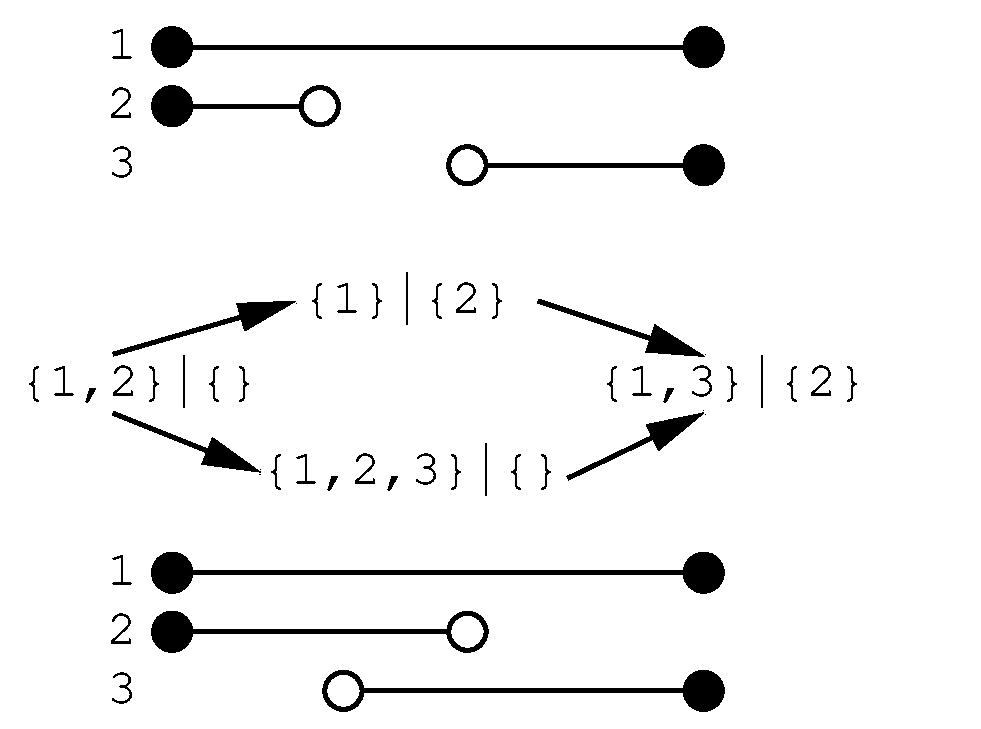
\includegraphics[width=0.9\columnwidth]{Fig1.eps}
  \end{center}
  \caption{Schematic representation of the breakpoint alignment model of
    \cite{AlArab:17a}, with global reference sequence $\mathtt{1}$,
    right-local prefix $\mathtt{2}$, and left-local suffix $\mathtt{3}$.
    The initial and terminal states of valid alignments are therefore
    $A|D=\{\mathtt{1},\mathtt{2}\}|\{\}$ and
    $\{\mathtt{1},\mathtt{3}\}|\{\mathtt{2}\}$, respectively.  There are
    two distinct path of transitioning between these states with
    intermediates states $\{\mathtt{1}\}|\{\mathtt{2}\}$ (if $\mathtt{2}$
    and $\mathtt{3}$ do not overlap) and $\{\mathtt{1,2,3}\}|\{\}$ (if
    $\mathtt{2}$ and $\mathtt{3}$ overlap in their aligned part). The black
    bullets indicate that the correspond end of the sequence is present in
    the alignment, open circles indicate the prefixes of suffixes remain
    unaligned.}
  \label{fig:Marwa}
\end{figure}


In a quite general form (which uses the usual heuristic version of the
affine gap cost model), the recursion for the optimal alignment score are
of the form
\begin{equation} 
  S^{\pi,(A,D)}_I = \max 
      \begin{cases}
        \displaystyle\max_{\tau} 
            \left[ S^{\tau,(A,D)}_{I-\pi} + s(\tau\to\pi)
                    \right]
        \\
        \displaystyle\max_{(A',D')\pprec(A,D)}  
                    \left[ S^{\pi,(A,D)}_I + s^*\right]
       \end{cases} 
\label{eq:maxrec}
\end{equation}
The upper multi-index $\pi$ (a non-null binary vector) denotes gap pattern
in the last alignment column, the lower multi-index $I$ describes the
length of the prefix included in the alignment up to this column. The
scoring function $s(\,.\,)$ in the most general form depends on both gap
patterns as well as the actual sequence entries. The second alternative
does not move in the alignment but changes the state, a step that may also
be associated with a cost $s^*$, which in the most general case may depend
on $I,\pi,A,D,A',D'$.  We note that the recursion simplifies in the case of
additive scores. In this case $S$ does not depend on the gap pattern and
$s$ becomes independent of $\tau$. The notation is illustrated in
Fig.~\ref{fig:Marwa} for the algorithm introduced in \cite{AlArab:17a}.
The full recursions for this model with affine gap costs are given in the
appendix of \cite{Retzlaff:18a}.


\section{\uppercase{Implementation}}

\TODO{FALCO should draft this: what exactly has been implemented} 


\section{\uppercase{Benchmark}}

\TODO{* describe benchmark data *}

\TODO{* what tools do we benchmark against, ans why? *} 


\section{\uppercase{Discussion}}
\section*{\uppercase{Acknowledgements}}

\noindent If any, should be placed before the references section
without numbering. To do so please use the following command:
\textit{$\backslash$section*\{ACKNOWLEDGEMENTS\}}


\vfill
\bibliographystyle{apalike}
{\small
\bibliography{implementGLOCAL}}


\section*{\uppercase{Appendix}}

\noindent If any, the appendix should appear directly after the
references without numbering, and not on a new page. To do so please use the following command:
\textit{$\backslash$section*\{APPENDIX\}}

\vfill
\end{document}




